% 第二章:导数与微分
\chapter{导数与微分}
\section{导数的定义}
\begin{example}{}{}
    已知$x,y>0$,且$x^2+9y^2=12$,则$\dfrac{x+2}{y+1}-3x$的最小值为\underline{\hspace{2cm}}.
\end{example}
\begin{solution}

\end{solution}
\newpage
\begin{example}{(高考题改编)}{}
    (单选)设代数式$\displaystyle T = \dfrac21\cdot\dfrac{4}{3}\cdot\dfrac{6}{5}\cdots\dfrac{200}{199}$,则(~~~~)

    \begin{tabular}{@{}llll@{}}
        A.$14< T < 16$&B.$16 < T < 18$&C.$18< T < 20$&D.$20< T < 22$
    \end{tabular}
\end{example}
\begin{solution}
    出题背景是大名鼎鼎的Wallis公式:
    \begin{align*}
I(n) = \int_0^{\frac{\pi}{2}} \sin^n x \, \mathrm{d}x 
&= \int_0^{\frac{\pi}{2}} \sin^{n-1} x \, \mathrm{d}(-\cos x) \\
&= (-\cos x \sin^{n-1} x) \rvert_{0}^{\frac{\pi}{2}} - \int_{0}^{\frac{\pi}{2}} (-\cos x) \, \mathrm{d}\sin^{n-1} x \\
&= (-\cos x \sin^{n-1} x) |_0^{\frac{\pi}{2}} - \int_0^{\frac{\pi}{2}} (-\cos^2 x) (n-1) \sin^{n-2} x \, \mathrm{d}x \\
&= (n-1) \int_0^{\frac{\pi}{2}} (\sin^{n-2} x - \sin^n x) \, \mathrm{d}x 
= (n-1) I(n-2) - (n-1) I(n) \\
\Rightarrow I(n) = \frac{n-1}{n} I(n-2) 
&\Rightarrow 
\begin{cases}
\dfrac{I(2n+1)}{I(2n-1)} = \dfrac{2n}{2n+1} \\
\dfrac{I(2n)}{I(2n-2)} = \dfrac{2n-1}{2n}
\end{cases}
\end{align*}
所以累乘有:
\begin{align*}
    \dfrac{I(3)}{I(1)} \cdot \dfrac{I(5)}{I(3)} \cdots \dfrac{I(2n+1)}{I(2n-1)} &= \dfrac{2 \times 1}{2 \times 1 + 1} \times \dfrac{2 \times 2}{2 \times 2 + 1} \times \cdots \times \dfrac{2n}{2n + 1} = \dfrac{(2n)!!}{(2n + 1)!!}\\
    \dfrac{I(2)}{I(0)} \cdot \dfrac{I(4)}{I(2)} \cdots \dfrac{I(2n)}{I(2n - 2)} &= \dfrac{2 \times 1 - 1}{2 \times 1} \times \dfrac{2 \times 2 - 1}{2 \times 2} \times \cdots \times \dfrac{2n - 1}{2n} = \dfrac{(2n - 1)!!}{(2n)!!}\end{align*}
又因为:
\begin{align*}
I(2k+1)<I(2k)<I(2k-1)&\Rightarrow \frac{(2k)!!}{(2k+1)!!}<\frac{(2k-1)!!}{(2k)!!}\frac{\pi}{2}<\frac{(2k-2)!!}{(2k-1)!!} \\&\Rightarrow \frac{1}{2k+1}\cdot[\frac{(2k)!!}{(2k-1)!!}]^{2}<\frac{\pi}{2}<\frac{1}{2k}\cdot[\frac{(2k)!!}{(2k-1)!!}]^{2}
\end{align*}\vspace{-10pt}
\[\Rightarrow \frac{\pi}{2}=\prod_{n=1}^\infty\frac{4n^2}{4n^2-1}=\prod_{n=1}^\infty(\frac{2n}{2n+1}\cdot\frac{2n}{2n-1})=(\frac{2}{1}\cdot\frac{2}{3})\cdot(\frac{4}{3}\cdot\frac{4}{5})\cdot(\frac{6}{5}\cdot\frac{6}{7})(\frac{8}{7}\cdot\frac{8}{9})\]
所以:
    \begin{align*}
        T^2=&\dfrac21\cdot\dfrac21\cdot\dfrac{4}{3}\cdot\dfrac{4}{3}\cdot\dfrac{6}{5}\cdot\dfrac{6}{5}\cdots\dfrac{2n}{2n-1}\cdot\dfrac{2n}{2n-1}
        \approx\dfrac{\dfrac21\cdot\dfrac21\cdot\dfrac{4}{3}\cdot\dfrac{4}{3}\cdot\dfrac{6}{5}\cdot\dfrac{6}{5}\cdots\dfrac{2n}{2n-1}\cdot\dfrac{2n}{2n-1}}{(\dfrac{2}{1}\cdot\dfrac{2}{3})\cdot(\dfrac{4}{3}\cdot\dfrac{4}{5})\cdot(\dfrac{6}{5}\cdot\dfrac{6}{7})\cdots\dfrac{2n}{2n-1}\cdot\dfrac{2n}{2n+1}}\dfrac{\pi}{2}
    \end{align*}
则$T^2\approx\dfrac{(2n+1)\pi}{2}$,简单计算得知原题选B.
\newpage
方法二是使用放缩,先平方然后用糖水不等式,这个方法很套路,稍微一放就排除了A选项:
\begin{align*}T^{2}&=\frac{2}{1}\cdot\frac{2}{1}\cdot\frac{4}{3}\cdot\frac{4}{3}\cdot\frac{6}{5}\cdot\frac{6}{5}\cdots\frac{200}{199}\cdot\frac{200}{199}\\&>\frac{2}{1}\cdot\frac{2}{1}\cdot\frac{4}{3}\cdot\frac{5}{4}\cdot\frac{6}{5}\cdot\frac{7}{6}\cdots\frac{200}{199}\cdot\frac{201}{200}\\&=268>16^2\end{align*}
但是另一边就有点难度了,首先我们可以根据应试技巧,由“下界比较松”推测出来“上界比较紧”,所以在找上界的时候要放得仔细一点,当然严格说来这个推测逻辑缺乏依据。或者我们根据“仍有BCD选项需要分辨”的现状,可以考虑多保留几项再放缩,提高一下精度:
\begin{align*}T^2=&\frac{2}{1}\cdot\frac{2}{1}\cdot\frac{4}{3}\cdot\frac{4}{3}\cdots\frac{18}{17}\cdot\frac{18}{17}\cdot\frac{20}{19}\cdot\frac{20}{19}\cdot\frac{22}{21}\cdot\frac{22}{21}\cdot\frac{24}{23}\cdot\frac{24}{23}\cdots\frac{200}{199}\cdot\frac{200}{199}\\
    =&\frac{2}{1}\cdot\frac{2}{1}\cdot\frac{4}{3}\cdot\frac{4}{3}\cdots\frac{18}{17}\cdot\frac{18}{17}\cdot\frac{20}{19}\cdot\frac{20}{19}\cdot\frac{22}{21}\cdot\boxed{\frac{22}{21}}\cdot\frac{24}{23}\cdot\boxed{\frac{23}{22}}\cdots\frac{200}{199}\cdot\boxed{\frac{199}{198}}\\
    \Rightarrow T\leq&\frac{2}{1}\cdot\frac{4}{3}\cdot\frac{6}{5}\cdots\frac{20}{19}\cdot\sqrt{\frac{200}{20}}=\frac{512\times 512}{(15-4)(15-2)(15+2)(15+4)}\sqrt{10}\\
    =&\frac{262144}{46189}\sqrt{10}<3.1623\times5.68<18
\end{align*}
熟知$\sqrt{10}=3.16227766...<3.1623$,计算得到$\frac{262144}{46189}<5.68$这样得知本题选B.\newline 对于考试来说,把题目的答案改成$17<T<19$或许是更好的选择.
\end{solution}
\begin{example}{(高考题改编)}{}
    (单选)数列$a_{n}$各项为正整数且递增,$a_{n+2}=C_{a_{n+1}}^{a_{n}}$,则(~~~~~)

    \begin{tabular}{@{}ll@{}}
        A.$a_n<a_{n-1}+1$&B.$a_1,a_2,a_3$可能成等比数列\\
        C.$a_3a_4<a_5$&D.$a_3,a_4,a_5$可能成等比数列
    \end{tabular}
\end{example}
\begin{solution}
由于$a_n$递增,则A显然错误;下面考虑选项BD:
\[
    a_na_{n+2} = a_nC_{a_{n+1}}^{a_{n}}=a_{n+1}C_{a_{n+1}-1}^{a_{n}-1}=a_{n+1}^2\\\Rightarrow a_{n+1}=C_{a_{n+1}-1}^{a_{n}-1}
\]

当$a_n=1$时,代入表达式得到$a_{n+1}=C_{a_{n+1}-1}^{0}=1=a_n$,与数列递增矛盾;

当$a_n=2$时,代入表达式得到$a_{n+1}=C_{a_{n+1}-1}^{1}=a_{n+1}-1<a_{n+1}$,矛盾;

当$a_n>2$时,易得$a_{n+1}-1>2$,代入表达式得到
\[a_{n+1}=C_{a_{n+1}-1}^{a_{n}-1}\ge C_{a_{n+1}-1}^{2}=\dfrac{(a_{n+1}-1)(a_{n+1}-2)}{2}\]

解方程发现无整数解,而且由于$C_{a_{n+1}-1}^{1}=a_{n+1}-1$是小于$a_{n+1}$的最大整数,且有

\[C_{a_{n+1}-1}^{1}<C_{a_{n+1}-1}^{2},~~C_{a_{n+1}-1}^{2}\ne a_{n+1}\]

只可能是$C_{a_{n+1}-1}^{2}> a_{n+1}$.

雪上加霜的是,$C_{a_{n+1}-1}^{2}$和$C_{a_{n+1}-1}^{1}$中间没有数可以等于$C_{a_{n+1}-1}^{m}$,所以BD错误;

考虑C,易得$a_1\ne1,a_2\ge 4,a_3\ge6,a_4=C_{a_3}^{a_2}>2a_3+1$,由
\[a_5=C_{a_4}^{a_3}>a_3a_4 \Rightarrow a_3^2<C_{a_{4}-1}^{a_{3}-1}<C_{2a_3}^{a_3-1}\]

转化为$a_3^3+a_3<C_{2a_3}^{a_3}$这是显然成立的,故本题目选C
\end{solution}
\begin{example}{}{}
    已知$\triangle{ABC}$中,$A=3B=9C$,则$\cos A\cos B+\cos B\cos C+\cos C\cos A=$\underline{\hspace{1cm}}.
\end{example}
\begin{solution}
解得$A=\dfrac{9\pi}{13},B=\dfrac{3\pi}{13},C=\dfrac{\pi}{13}$考虑积化和差:
\begin{align*}
&\cos A\cos B+\cos B\cos C+\cos C\cos A\\
&=\dfrac12(\cos(A+B)+\cos(A-B)+\cos(B+C)+\cos(B-C)+\cos(A+C)+\cos(A+C))\\
&=\dfrac12(\cos\dfrac{12\pi}{13}+\cos\dfrac{6\pi}{13}+\cos\dfrac{4\pi}{13}+\cos\dfrac{2\pi}{13}+\cos\dfrac{10\pi}{13}+\cos\dfrac{8\pi}{13})\\
&=\dfrac{1}{2\sin\dfrac{\pi}{13}}\sin\dfrac{\pi}{13}(\cos\dfrac{2\pi}{13}+\cos\dfrac{4\pi}{13}+\cos\dfrac{6\pi}{13}+\cos\dfrac{8\pi}{13}+\cos\dfrac{10\pi}{13}+\cos\dfrac{12\pi}{13})\\
&=\dfrac{1}{4\sin\dfrac{\pi}{13}}(\sin\dfrac{\pi}{13}-\sin\dfrac{3\pi}{13}+\sin\dfrac{3\pi}{13}-\sin\dfrac{5\pi}{13}+\sin\dfrac{5\pi}{13}-\sin\dfrac{7\pi}{13}\\
&~~~~~~~~~~~~~~~~+\sin\dfrac{7\pi}{13}-\sin\dfrac{9\pi}{13}+\sin\dfrac{9\pi}{13}-\sin\dfrac{11\pi}{13}+\sin\dfrac{11\pi}{13}-\sin\dfrac{13\pi}{13})\\
&=-\dfrac14
\end{align*}
\end{solution}
\begin{theorem}{阿贝尔求和}{}
    设$B_n$是数列$b_n$的前$n$项和,当$n\ge 2$时,有:\vspace{-5pt}\[
    \sum_{i=1}^na_ib_i=a_nB_n-\sum_{i=1}^{n-1}(a_{i+1}-a_i)B_n\]
\end{theorem}
\begin{myproof}
    当$n\ge 2$时,有
    \begin{align*}
        \sum_{i=1}^na_ib_i=&a_1b_1+\sum_{i=2}^{n}a_i(B_i-B_{i-1})\\
        =&a_1b_1+\sum_{i=2}^{n}a_iB_i-\sum_{i=2}^{n}a_iB_{i-1}\\
        =&\sum_{i=1}^{n}a_iB_i-\sum_{i=1}^{n-1}a_{i+1}B_i\\
        =&a_nB_n-\sum_{i=1}^{n-1}(a_{i+1}-a_i)B_n
    \end{align*}
\end{myproof}
\begin{example}{(来自Fiddie)}{}
    设数列$\{a_n\}$的各项均为实数,且当$n\ge 2$时,$a_{n+1}+a_{n-1}=|a_n|$.证明:

    (1)存在大于$1$的正整数$m$使得$a_m\le 0$

    (2)存在正整数$m$使得$a_m\le 0,~a_{m+1}\le 0$

    (3)$a_n=a_{n+9}$ 
\end{example}
\begin{solution}
    (1)当$n\ge 2$时,由\[
    \begin{cases}a_{n+1}+a_{n-1}=|a_n|\\a_{n+2}+a_{n}=|a_{n+1}|\end{cases}\Rightarrow a_{n+2}+a_{n+1}+a_n+a_{n-1}=|a_n|+|a_{n+1}|
    \]\[
    \Rightarrow a_{n+2}+a_{n-1}=|a_n|-a_n+|a_{n+1}|-a_{n+1}\ge 0
    \]
    若$n\ge 2$时$a_n>0$,上式化为$a_{n+2}+a_{n-1}=0$,矛盾,故存在大于$1$的正整数$m$使得$a_m\le 0$
 
    \noindent(2)已证存在大于$1$的整数$m$使得$a_m\le 0$,现假设不存在正整数$k$使得$a_k\le 0,~a_{k+1}\le 0$,则不妨设$a_m$为首个小于等于$0$的项,由假设得$a_1,a_2,...a_{m-1}>0,a_m\le 0, a_{m+1}>0$,可以通过不断消元推出矛盾:\vspace{-10pt}
    \begin{align*}
    a_{m+1}+a_{m-1}=|a_m|&=-a_m\Rightarrow a_{m+1}=-a_m-a_{m-1}\\
    a_{m+2}+a_m=|a_{m+1}|&=a_{m+1}\Rightarrow a_{m+2}=a_{m+1}-a_m>0+0=0\\
    a_{m+3}+a_{m+1}=|a_{m+2}|&=a_{m+2}\Rightarrow a_{m+3}=a_{m+2}-a_{m+1}=a_{m+1}-a_m-a_{m+1}=-a_m\geq 0\\
    a_{m+4}+a_{m+2}=|a_{m+3}|&=-a_{m}\Rightarrow a_{m+4}=-a_{m}-a_{m+2}=-a_{m+1}<0\\
    a_{m+5}+a_{m+3}=|a_{m+4}|&=a_{m+1}\Rightarrow a_{m+5}=a_{m+1}-a_{m+3}=a_m+a_{m+1}=-a_{m-1}<0
    \end{align*}
    由$a_{m+4}<0,a_{m+5}<0$知矛盾,故存在正整数$k$使得$a_k\le 0,~a_{k+1}\le 0$.

\noindent(3)抓住上面第二小问的提示就可以得到:
    \vspace{-5pt}\begin{align*}
    a_{m+6}+a_{m+4}=|a_{m+5}|&=a_{m-1}\Rightarrow a_{m+6}=a_{m-1}-a_{m+4}=a_{m-1}+a_{m+1}=-a_m\\
    a_{m+7}+a_{m+5}=|a_{m+6}|&=-a_{m}\Rightarrow a_{m+7}=-a_{m}-a_{m+5}=a_{m-1}-a_m\\
    a_{m+8}+a_{m+6}=|a_{m+7}|&=a_{m-1}-a_m\Rightarrow a_{m+8}=a_{m-1}-a_m-a_{m+6}=a_{m-1}\\
    a_{m+9}+a_{m+7}=|a_{m+8}|&=a_{m-1}\Rightarrow a_{m+9}=a_{m-1}-a_{m+7}=a_{m-1}-a_{m-1}+a_{m}=a_m
    \end{align*}\vspace{-15pt}
    所以设$T=9$,有\[\begin{cases}a_{m}=a_{m+nT},n\in N\\a_{m-1}=a_{m-1+nT},n\in N\end{cases}\]
    然后由于\[a_{m-2+nT}=|a_{m-1+nT}|-a_{m+nT}=|a_{m-1}|-a_{m}=a_{m-2}\]以此类推,则有\[
    a_k=a_{k+nT},k\in N_+,k\leq m\]取合适的$m$使得$m$大于$T$,则数列$\{a_n\}$为周期数列,其中一个周期为9
\end{solution}
\begin{example}{(南通9调14题)}{}
    已知$x,y$满足$(\sqrt{x^2+1}-x)(\sqrt{y^2+4}-y)=2$,则$4^{x}+2^{y-1}$的最小值为\underline{\hspace{1cm}}.
\end{example}
\begin{solution}
    套路题,先换元:\[
    \begin{cases}
        m=\sqrt{x^2+1}-x\Rightarrow x=\dfrac{1}{2m}-\dfrac{2}{m}\\[8pt]
        n=\sqrt{y^2+4}-y\Rightarrow y=\dfrac{2}{n}-\dfrac{n}{2}\end{cases}
    \]
    再代入$mn=2\Rightarrow n=\dfrac{2}{m}$:
    \[y=\dfrac{2}{n}-\dfrac{n}{2}=m-\dfrac{1}{m}\Rightarrow y=-2x\]
    所以:\[4^{x}+2^{y-1}=4^{x}+\dfrac{1}{2\times 4^x}\geq 2\sqrt{\dfrac{1}{2}}=\sqrt2\]当$x=\frac14$时取得等号
\end{solution}
\newpage
\begin{example}{(深圳中学2025届二轮一阶)}{}
    \noindent$\triangle{ABC}$中,若
    \[\begin{cases}\overrightarrow{AD}=\dfrac{\lambda}{\lambda+1}\overrightarrow{AC}\\
        \overrightarrow{AE}=\dfrac{\mu}{\mu+1}\overrightarrow{AB}\end{cases}\]
    \noindent 则连接$BD,CE$得到交点$Q$,任取$\triangle{ABC}$所在平面内某一点$P$,那么有:\[
    PQ^2=\dfrac{PA^2+\mu PB^2+\lambda PC^2}{1+\lambda+\mu}-\dfrac{\lambda\mu BC^2+\lambda AC^2+\mu AB^2}{\left(1+\lambda+\mu\right)^2}
    \]
\end{example}
\begin{solution}
      设\[
      \begin{cases}\overrightarrow{AQ}=x\overrightarrow{AD}+(1-x)\overrightarrow{AB}=x\dfrac{\lambda}{1+\lambda}\overrightarrow{AC}+(1-x)\overrightarrow{AB}\\[10pt]
      \overrightarrow{AQ}=y\overrightarrow{AE}+(1-y)\overrightarrow{AC}=y\dfrac{\mu}{1+\mu}\overrightarrow{AB}+(1-y)\overrightarrow{AC}\end{cases}\Rightarrow \begin{cases}x=\dfrac{\lambda+1}{1+\lambda+\mu}\\[8pt]y=\dfrac{\mu+1}{1+\lambda+\mu}\end{cases}
      \]
      化为形如$x\overrightarrow{QA}+y\overrightarrow{QB}+z\overrightarrow{QC}=0$的方程:
      \begin{align*}
          \Rightarrow \overrightarrow{AQ}&=\dfrac{\lambda}{1+\lambda+\mu}\overrightarrow{AC}+\dfrac{\mu}{1+\lambda+\mu}\overrightarrow{AB}\\
          &=\dfrac{\lambda}{1+\lambda+\mu}(\overrightarrow{AQ}+\overrightarrow{QC})+\dfrac{\mu}{1+\lambda+\mu}(\overrightarrow{AQ}+\overrightarrow{QB})\\
          &=\dfrac{\lambda+\mu}{1+\lambda+\mu}\overrightarrow{AQ}+\dfrac{\lambda}{1+\lambda+\mu}\overrightarrow{QC}+\dfrac{\mu}{1+\lambda+\mu}\overrightarrow{QB}\\
          \Rightarrow \overrightarrow{QA}&+\lambda\overrightarrow{QC}+\mu\overrightarrow{QB}=\vec{0}\\
          \Rightarrow \overrightarrow{PA}&-\overrightarrow{PQ}+\lambda(\overrightarrow{PC}-\overrightarrow{PQ})+\mu(\overrightarrow{PB}-\overrightarrow{PQ})=\vec{0}\\
          \Rightarrow \overrightarrow{PA}&+\lambda\overrightarrow{PC}+\mu\overrightarrow{PB}=(1+\lambda+\mu)\overrightarrow{PQ}
      \end{align*}
    平方得:\[
PA^2+\lambda^2PC^2+\mu^2PB^2+2\lambda\overrightarrow{PA}\cdot\overrightarrow{PC}+2\mu\overrightarrow{PA}\cdot\overrightarrow{PB}+2\lambda\mu\overrightarrow{PC}\cdot\overrightarrow{PB}=(1+\lambda+\mu)^2PQ^2\]分别
代入\[\begin{cases}2\lambda\overrightarrow{PA}\cdot\overrightarrow{PC}=\lambda\bigg(PA^2+PC^2-(\overrightarrow{PA}-\overrightarrow{PC})\bigg)^2=\lambda(PA^2+PC^2-AC^2)\\
    2\mu\overrightarrow{PA}\cdot\overrightarrow{PB}=\mu\bigg(PA^2+PB^2-(\overrightarrow{PA}-\overrightarrow{PB})\bigg)^2=\mu(PA^2+PB^2-AB^2)\\
    2\lambda\mu\overrightarrow{PC}\cdot\overrightarrow{PB}=\lambda\mu\bigg(PC^2+PB^2-(\overrightarrow{PC}-\overrightarrow{PB})\bigg)^2=\lambda\mu(PC^2+PB^2-BC^2)
\end{cases}\]
    变形即可得到:\[
    PQ^2=\dfrac{PA^2+\mu PB^2+\lambda PC^2}{1+\lambda+\mu}-\dfrac{\lambda\mu BC^2+\lambda AC^2+\mu AB^2}{\left(1+\lambda+\mu\right)^2}\]
\end{solution}
因此有结论:
\begin{conclusion}{结论}{}
    \noindent 平面内给定$\triangle{ABC}$,若点$Q$满足\vspace{-10pt}
    \[\overrightarrow{QA}+\lambda\overrightarrow{QC}+\mu\overrightarrow{QB}=\vec{0}\vspace{-10pt}\]则任取$\triangle{ABC}$所在平面内某一点$P$,有\[PQ^2=\dfrac{PA^2+\mu PB^2+\lambda PC^2}{1+\lambda+\mu}-\dfrac{\lambda\mu BC^2+\lambda AC^2+\mu AB^2}{\left(1+\lambda+\mu\right)^2}\]
\end{conclusion}
\begin{example}{奔驰定理}{}
    \noindent 已知平面直角坐标系$xOy$中有一个$\triangle{ABC}$,以及平面内任意一点$P$,则有:\[
    \begin{vmatrix}
    x_B & y_B & 1\\
    x_C & y_C & 1\\
    x_P & y_P & 1\\
\end{vmatrix}\overrightarrow{PA}+\begin{vmatrix}
    x_C & y_C & 1\\
    x_A & y_A & 1\\
    x_P & y_P & 1\\
\end{vmatrix}\overrightarrow{PB}+\begin{vmatrix}
    x_A & y_A & 1\\
    x_B & y_B & 1\\
    x_P & y_P & 1\\
\end{vmatrix}\overrightarrow{PC}=\vec{0}\]
这等价于\[S_{\triangle{PBC}}\overrightarrow{PA}+S_{\triangle{PAC}}\overrightarrow{PB}+S_{\triangle{PAB}}\overrightarrow{PC}=\vec{0}\]
这里的三角形面积是有向面积,我们必须在计算三角形面积时按照字母顺序看一下方向(顺时针或逆时针),然后将与其他两个方向不同的三角形的对应面积取负值。
\end{example}
\begin{solution}

\end{solution}
\begin{example}{外心向量关系}{}
    已知平面直角坐标系$xOy$中有一个$\triangle{ABC}$,则其外心满足关系式:
\end{example}
\begin{solution}

\end{solution}
\begin{example}{三角形外心坐标}{}
    已知平面直角坐标系$xOy$中有一个$\triangle{ABC}$,则其外心的坐标为\[
    \left(\dfrac{\begin{vmatrix}
    OA^2 & y_A & 1\\
    OB^2 & y_B & 1\\
    OC^2 & y_C & 1\\
\end{vmatrix}}{2\begin{vmatrix}
    x_A & y_A & 1\\
    x_B & y_B & 1\\
    x_C & y_C & 1\\
\end{vmatrix}},\dfrac{\begin{vmatrix}
    x_A & OA^2 & 1\\
    x_B & OB^2 & 1\\
    x_C & OC^2 & 1\\
\end{vmatrix}}{2\begin{vmatrix}
    x_A & y_A & 1\\
    x_B & y_B & 1\\
    x_C & y_C & 1\\
\end{vmatrix}}\right)
\]\end{example}
\begin{solution}

\end{solution}
\begin{example}{三角形垂心坐标}{}
    已知平面直角坐标系$xOy$中有一个$\triangle{ABC}$,则其垂心的坐标为\[
    \left(\dfrac{\begin{vmatrix}
    x_Bx_C+y_By_C & y_A & 1\\
    x_Ax_C+y_Ay_C & y_B & 1\\
    x_Ax_B+y_Ay_B & y_C & 1\\
    \end{vmatrix}}{-\begin{vmatrix}
    x_A & y_A & 1\\
    x_B & y_B & 1\\
    x_C & y_C & 1\\
    \end{vmatrix}},\dfrac{\begin{vmatrix}
    x_A & x_Bx_C+y_By_C & 1\\
    x_B & x_Ax_C+y_Ay_C & 1\\
    x_C & x_Ax_B+y_Ay_B & 1\\
    \end{vmatrix}}{-\begin{vmatrix}
    x_A & y_A & 1\\
    x_B & y_B & 1\\
    x_C & y_C & 1\\
    \end{vmatrix}}\right)\]
\end{example}
\begin{solution}
\end{solution}
\begin{example}{三角形的内心坐标}{}
    已知平面直角坐标系$xOy$中有一个$\triangle{ABC}$,则其内心的坐标为\[
    \left(\dfrac{ax_A+bx_B+cx_C}{a+b+c},\dfrac{ay_A+by_B+cy_C}{a+b+c}\right)
    \]
\end{example}
\begin{solution}

\end{solution}
\begin{example}{容斥原理练习}{}
    某学校举办比赛,有$20$个参赛名额,现在分给$4$个不同的班,保证至少有一个班的名额为$4$个,且每一个班都有名额,则共有\underline{\hspace{1cm}}种分法。
\end{example}
\begin{solution}
    设四个班的名额为$x_1,x_2,x_3,x_4\in N_+$,则分法数就是集合$A_i=\{(x_1,x_2,x_3,x_4)|x_i=4,x_1+x_2+x_3+x_4=20\}$的元素个数,又因为
    \begin{align*}|A_{1}|&=\{(x_{1},x_{3},x_{4})\mid x_{2}+x_{3}+x_{4}=16,x_{2},x_{3},x_{4}>0\}=C_{15}^{2}\\|A_{1}\cap A_{2}|&=\{(x_{3},x_{4})\mid x_{3}+x_{4}=12,x_{3},x_{4}>0\}=C_{11}^{1}\\|A_{1}\cap A_{2}\cap A_{3}|&=1\\
    |A_1\cup A_2\cup A_3\cup A_4|&=C_4^1|A_1|-C_4^2|A_1\cap A_2|+C_4^3|A_1\cap A_2\cap A_3|\\
        &=C_4^1C_{15}^2-C_4^2+C_4^3C_{11}^1=358\end{align*}
\end{solution}
\newpage
\begin{example}{求和}{}
    计算$\displaystyle \sum_{i=0}^{n-1}(-1)^{i}C_{n-1}^{i}(i+1)^k$,其中$k<n-1,k\in N_+$
\end{example}
\begin{solution}
    定义函数并对其求$k$阶导数:\begin{align*}f(x)=&\displaystyle\sum_{i=0}^{n-1}(-1)^{i}C_{n-1}^{i}x^{i+1}
        =\displaystyle x\sum_{i=0}^{n-1}(-x)^{i}C_{n-1}^{i}\\
        =&\displaystyle x(1-x)^{n-1}
        =(x-1+1)(1-x)^{n-1}
        =(1-x)^{n-1}-(1-x)^n\\
    \Rightarrow f(1)=&\displaystyle\sum_{i=0}^{n-1}(-1)^{i}C_{n-1}^{i}=0\\
     f^{(k)}(x)=&\displaystyle\sum_{i=0}^{n-1}(-1)^{i}C_{n-1}^{i}A_{i+1}^{k}x^{i+1-k}\Rightarrow
     f^{(k)}(1)=\displaystyle\sum_{i=0}^{n-1}(-1)^{i}C_{n-1}^{i}A_{i+1}^{k}
    \end{align*}
    现已很接近原式,问题在于沟通$A_{i+1}^{k}$和${(i+1)}^{k}$,我们假想这样一个情境:有$k$个不同的球等待放进$i+1$个不同的盒子里面,放置过程中允许空盒的存在,所以放法是${(i+1)}^{k}$,然后我们换一种方式,考虑分为恰好有$0,1,2,3,4,...,k$个非空盒子的情况,那么求和就是\[\sum_{r=0}^kS(k,r)r!C_{i+1}^r=\sum_{r=0}^kS(k,r)A_{i+1}^r\]
    其中$S(k,r)$表示$k$个有标号的球放到r个同样的盒子里面的方法数,$C_{i+1}^r$表示从$i+1$个不同的盒子无序地挑出$r$个盒子来放球,再对其进行全排列使得挑出来的$r$个盒子有编号,则:\[(i+1)^{k}=\sum_{r=0}^kS(k,r)A_{i+1}^r
    \]
    那么代入到$\displaystyle \sum_{i=0}^{n-1}(-1)^{i}C_{n-1}^{i}(i+1)^k$中就有:\begin{align*}
    \sum_{i=0}^{n-1}(-1)^{i}C_{n-1}^{i}(i+1)^k=&\sum_{i=0}^{n-1}\bigg((-1)^{i}C_{n-1}^{i}\bigg(\sum_{r=0}^kS(k,r)A_{i+1}^r\bigg)\bigg)\\=&\sum_{i=0}^{n-1}\sum_{r=0}^kS(k,r)A_{i+1}^r(-1)^{i}C_{n-1}^{i}\\=&\sum_{r=0}^k\sum_{i=0}^{n-1}S(k,r)A_{i+1}^r(-1)^{i}C_{n-1}^{i}=\sum_{r=0}^kS(k,r)f^{(r)}(1)
    \end{align*}
    对$(1-x)^{n-1}-(1-x)^n$求导易得$f(x)$只有第$n-1$和$n$阶导数在$x=1$处的值不是$0$,即:\[\sum_{i=0}^{n-1}(-1)^{i}C_{n-1}^{i}(i+1)^k=0
    \]
\end{solution}
\begin{example}{证明}{}
    \vspace{-15pt}\begin{align*}
    (1)\quad&\frac{\sin B - \cos A}{\sin A + \cos B} - \frac{\sin A + \cos B}{\sin B - \cos A} = 2\tan(A+B)\\
    (2)\quad&\frac{\sin B - \cos A}{\sin A - \cos B} - \frac{\sin A - \cos B}{\sin B - \cos A} = \frac{\cos B + \sin A}{\cos A + \sin B} - \frac{\cos A + \sin B}{\cos B + \sin A} = 2\tan(A-B)\\
    (3)\quad&\frac{\cos A - \cos B}{\sin A - \sin B} - \frac{\sin A - \sin B}{\cos A - \cos B} = 2\cot(A+B)\\
    (4)\quad&\frac{\cos A - \cos B}{\sin A + \sin B} - \frac{\sin A + \sin B}{\cos A - \cos B} = \frac{\cos A + \cos B}{\sin A - \sin B} - \frac{\sin A - \sin B}{\cos A + \cos B} = 2\cot(A-B)\end{align*}
\end{example}
\begin{solution}
第一种方法就是通分,拿一个式子举例
\begin{align*}
&\dfrac{\sin B - \cos A}{\sin A - \cos B} - \dfrac{\sin A - \cos B}{\sin B - \cos A}\\[1.2ex]
&=\dfrac{(\sin B - \cos A)^2 - (\sin A - \cos B)^2}{(\sin B - \cos A)\left(\sin A - \cos B\right)}\\[1.2ex]
&=\dfrac{\sin^2 B - 2\sin B \cos A + \cos^2 A - \sin^2 A + 2\sin A \cos B - \cos^2 B}{\sin B \sin A - \sin A \cos A - \sin B \cos B + \cos B \cos A}\\[1.2ex]
&=\dfrac{\cos 2A - \cos 2B + 2\left(\sin A \cos B - \sin B \cos A\right)}{\cos\left(A - B\right) - \dfrac{1}{2}\left(\sin 2A + \sin 2B\right)}\\[1.2ex]
&=\dfrac{-2\sin\left(A + B\right)\sin\left(A - B\right) + 2\sin\left(A - B\right)}{\cos\left(A - B\right) - \sin\left(A + B\right)\cos\left(A - B\right)}
=\dfrac{2\left[1 - \sin\left(A + B\right)\right]\sin\left(A - B\right)}{\left[1 - \sin\left(A + B\right)\right]\cos\left(A - B\right)}
\\[1.2ex]&=\dfrac{2\sin\left(A - B\right)}{\cos\left(A - B\right)} = 2\tan\left(A - B\right).
\end{align*}
再写一个:
\begin{align*}
&\dfrac{\cos A - \cos B}{\sin A - \sin B} - \dfrac{\sin A - \sin B}{\cos A - \cos B}\\[1.2ex]
&=\dfrac{(\cos A - \cos B)^2 - (\sin A - \sin B)^2}{(\cos A - \cos B)(\sin A - \sin B)}\\[1.2ex]
&=\dfrac{\cos^2 A - 2\cos A\cos B + \cos^2 B - \sin^2 A + 2\sin A\sin B - \sin^2 B}{\sin A\cos A - \sin A\cos B - \sin B\cos A + \sin B\cos B}\\[1.2ex]
&=\dfrac{(\cos^2 A - \sin^2 A) + (\cos^2 B - \sin^2 B) - 2\cos A\cos B + 2\sin A\sin B}{\sin A\cos A + \sin B\cos B - (\sin A\cos B + \sin B\cos A)}\\[1.2ex]
&=\dfrac{\cos 2A + \cos 2B - 2\cos(A + B)}{\dfrac{1}{2}(\sin 2A + \sin 2B) - \sin(A + B)}
=\dfrac{2\cos(A + B)\cos(A - B) - 2\cos(A + B)}{\sin(A + B)\cos(A - B) - \sin(A + B)}\\[1.2ex]
&=\dfrac{2\cos(A + B)[\cos(A - B) - 1]}{\sin(A + B)[\cos(A - B) - 1]}
=\dfrac{2\cos(A + B)}{\sin(A + B)} = 2\cot(A + B).
\end{align*}
第二种方法就是按部就班地和差化积,拿一个式子举例
\begin{align*}
&\dfrac{\sin B - \cos A}{\sin A - \cos B} - \dfrac{\sin A - \cos B}{\sin B - \cos A}\\[1.2ex]
&=\dfrac{\cos\left(\dfrac{\pi}{2} - B\right) - \cos A}{\sin A - \sin\left(\dfrac{\pi}{2} - B\right)} - \dfrac{\sin A - \sin\left(\dfrac{\pi}{2} - B\right)}{\cos\left(\dfrac{\pi}{2} - B\right) - \cos A}\\[1.2ex]
&=\dfrac{-2\sin\left(\dfrac{\pi}{4} + \dfrac{A - B}{2}\right)\sin\left(\dfrac{\pi}{4} - \dfrac{A + B}{2}\right)}{2\cos\left(\dfrac{\pi}{4} + \dfrac{A - B}{2}\right)\sin\left(\dfrac{A + B}{2} - \dfrac{\pi}{4}\right)} - \dfrac{2\cos\left(\dfrac{\pi}{4} + \dfrac{A - B}{2}\right)\sin\left(\dfrac{A + B}{2} - \dfrac{\pi}{4}\right)}{-2\sin\left(\dfrac{\pi}{4} + \dfrac{A - B}{2}\right)\sin\left(\dfrac{\pi}{4} - \dfrac{A + B}{2}\right)}\\[1.2ex]
&=\dfrac{\sin\left(\dfrac{\pi}{4} + \dfrac{A - B}{2}\right)}{\cos\left(\dfrac{\pi}{4} + \dfrac{A - B}{2}\right)} - \dfrac{\cos\left(\dfrac{\pi}{4} + \dfrac{A - B}{2}\right)}{\sin\left(\dfrac{\pi}{4} + \dfrac{A - B}{2}\right)} = \dfrac{\sin^2\left(\dfrac{\pi}{4} + \dfrac{A - B}{2}\right) - \cos^2\left(\dfrac{\pi}{4} + \dfrac{A - B}{2}\right)}{\sin\left(\dfrac{\pi}{4} + \dfrac{A - B}{2}\right)\cos\left(\dfrac{\pi}{4} + \dfrac{A - B}{2}\right)}\\[1.2ex]
&=-2\dfrac{\cos\left[2 \cdot \left(\dfrac{\pi}{4} + \dfrac{A - B}{2}\right)\right]}{\sin\left[2 \cdot \left(\dfrac{\pi}{4} + \dfrac{A - B}{2}\right)\right]} = -2\dfrac{\cos\left(\dfrac{\pi}{2} + A - B\right)}{\sin\left(\dfrac{\pi}{2} + A - B\right)}\\[1.2ex]
&=-2\dfrac{-\sin\left(A - B\right)}{\cos\left(A - B\right)} = 2\tan\left(A - B\right).
\end{align*}
再写一个:
\begin{align*}
&\dfrac{\cos A - \cos B}{\sin A - \sin B} - \dfrac{\sin A - \sin B}{\cos A - \cos B}\\[1.2ex]
&=\dfrac{\sin\left(\dfrac{A+B}{2}\right)\sin\left(\dfrac{A-B}{2}\right)}{\cos\left(\dfrac{A+B}{2}\right)\sin\left(\dfrac{A-B}{2}\right)} - \dfrac{\cos\left(\dfrac{A+B}{2}\right)\sin\left(\dfrac{A-B}{2}\right)}{\sin\left(\dfrac{A+B}{2}\right)\sin\left(\dfrac{A-B}{2}\right)}\\[1.2ex]
&=\dfrac{\sin\left(\dfrac{A+B}{2}\right)}{\cos\left(\dfrac{A+B}{2}\right)} - \dfrac{\cos\left(\dfrac{A+B}{2}\right)}{\sin\left(\dfrac{A+B}{2}\right)} = \dfrac{\sin^2\left(\dfrac{A+B}{2}\right) - \cos^2\left(\dfrac{A+B}{2}\right)}{\sin\left(\dfrac{A+B}{2}\right)\cos\left(\dfrac{A+B}{2}\right)}\\[1.2ex]
&=-\dfrac{\cos\left[2 \cdot \dfrac{A+B}{2}\right]}{\dfrac{1}{2}\sin\left[2 \cdot \dfrac{A+B}{2}\right]} = -\dfrac{\cos(A+B)}{\dfrac{1}{2}\sin(A+B)}\\[1.2ex]
&=-2\dfrac{\cos(A+B)}{\sin(A+B)} = 2\cot(A+B).
\end{align*}
\end{solution}
\newpage
\begin{example}{(2008年江西浸泡压轴题)}{}
    已知$\displaystyle f \left( x \right)= \frac{1}{ \sqrt{1+x}}+ \frac{1}{ \sqrt{1+a}}+ \sqrt{ \frac{ax}{ax+8}},x \in \left( 0,+ \infty \right)$
\vspace{5pt}

    (1)当$a=8$时,求$f(x)$的单调区间.

    (2)对于任意正数$a$,求证$1<f(x)<2$.
\end{example}
\begin{solution}
    (1)当$a=8$时,$\displaystyle f(x)= \frac{1}{ \sqrt{1+x}}+ \frac{1}{3}+ \sqrt{ \frac{x}{x+1}}$,观察式子不难想到换元$x=\tan^2\theta$:
    \[f(x)=\frac{1}{ \sqrt{1+\tan^2\theta}}+ \frac{1}{3}+ \sqrt{ \frac{\tan^2\theta}{\tan^2\theta+1}}\\=\cos \theta+ \frac{1}{3}+ \sin \theta\\=\sqrt{2}\sin(\theta+\frac{\pi}{4})+\frac13\]
    由$\theta\in(0,\frac{\pi}{2})$,所以$\sin(\theta+\frac{\pi}{4})$在$(0,\frac{\pi}{4})$上单调递增,在$(\frac{\pi}{4},\frac{\pi}{2})$上单调递减,所以$f(x)$在$(0,1)$上单调递增,在$(1,+\infty)$上单调递减。

    (2)这道题难就难在题目给了函数,似乎是暗示学生走求导的路子,但求导异常难做,反而看成是不等式问题却能找到方向。由于函数结构不对称,我们引入第三个变元就可以将本题条件化为对称形式:令$f \left( x \right)= \frac{1}{ \sqrt{1+x}}+ \frac{1}{ \sqrt{1+y}}+ \sqrt{ \frac{xy}{xy+8}},x,y \in \left( 0,+ \infty \right)$:
    \[
    \begin{cases}a=\dfrac{1}{\sqrt{1+x}}\in(0,1)\\b=\dfrac{1}{ \sqrt{1+y}}\in(0,1)\\c=\sqrt{ \dfrac{xy}{xy+8}}\in(0,1)\end{cases}\Rightarrow 
    \begin{cases}a^2=\dfrac{1}{1+x},x=\dfrac{1}{a^2}-1\\[1.2ex]b^2=\dfrac{1}{1+y},y=\dfrac{1}{b^2}-1\\[1.2ex]c^2=\dfrac{ax}{ax+8}=1-\dfrac{8}{ax+8}\end{cases}
    \]
现在要找到三个元之间的关系式,消元法就够了:
\[
c^2=1-\dfrac{8}{ax+8}=1-\dfrac{8}{(\dfrac{1}{a^2}-1)(\dfrac{1}{b^2}-1)+8}\Rightarrow (1-a^2)(1-b^2)(1-c^2)=8a^2b^2c^2
\]先假设$a+b+c>=2$,列出已知条件:
\[\begin{cases}a,b,c\in(0,1),\quad a+b+c\geq 2\\(1-a^2)(1-b^2)(1-c^2)=8a^2b^2c^2\end{cases}\]
我们现在要证明的是“同时满足这几个条件的题目是一个错题”。其中最后一个条件看似很强,给出了三元关系,但是如果不拿来消元的话很难用上,而消元又回到了原题的情形,这就很尴尬了。那我们不妨尝试删除$(1-a^2)(1-b^2)(1-c^2)=8a^2b^2c^2$并尝试通过剩余条件导出$(1-a^2)(1-b^2)(1-c^2)\ne8a^2b^2c^2$,即$(1-a^2)(1-b^2)(1-c^2)>8a^2b^2c^2$或$(1-a^2)(1-b^2)(1-c^2)<8a^2b^2c^2$。而这个式子是对称的,我们不妨拆成$(1-a^2)>2bc$或$(1-a^2)<2bc$来证明,虽然这个转换之后的式子是原来式子成立的充分而非必要条件,但确实是可以尝试的方向,是不是可以叫“充分性探路”呢?
\[\begin{cases}1-a^2=(1-a)(1+a)<2(1-a)=2(b+c-1)\\(1-b)(1-c)\in(0,1)\Rightarrow bc+1<b+c\end{cases}\Rightarrow 1-a^2<2bc\]
这样同理得到$1-b^2<2ac,1-c^2<2ab$,这样就有$(1-a^2)(1-b^2)(1-c^2)<8a^2b^2c^2$,矛盾,所以$a+b+c<2$。然后我们紧接着设$a+b+c\leq 1$,同样列出已知条件:
\[\begin{cases}a,b,c\in(0,1),\quad a+b+c<=1\\(1-a^2)(1-b^2)(1-c^2)=8a^2b^2c^2\end{cases}\]
同样的套路,我们依然考虑证明$(1-a^2)>2bc$或$(1-a^2)<2bc$,由
\[\begin{cases}1-a^2=(1-a)(1+a)>1-a\geq b+c\\(1-b)(1-c)\in(0,1)\Rightarrow bc<b+c\end{cases}\Rightarrow 1-a^2>2bc\]
这样同理得到$1-b^2>2ac,1-c^2>2ab$,这样就有$(1-a^2)(1-b^2)(1-c^2)>8a^2b^2c^2$,矛盾。所以只能是$1<a+b+c<2$.

\noindent(3)当然本题解法不唯一,比如说我们根据
\[f \left( x \right)= \frac{1}{ \sqrt{1+x}}+ \frac{1}{ \sqrt{1+y}}+ \sqrt{ \frac{xy}{xy+8}}=\frac{1}{ \sqrt{1+x}}+ \frac{1}{\sqrt{1+y}}+ \frac{1}{1+\sqrt{\frac{8}{xy}}}\]
来换元$z=\dfrac{8}{xy}$,则有$xyz=8$要证明$ 1<\dfrac{1}{ \sqrt{1+x}}+ \dfrac{1}{ \sqrt{1+y}}+ \dfrac{1}{\sqrt{1+z}}<2$,已知条件是$x,y,z>0$,那么$(x-2)(y-2)(z-2)<8$,不妨假设数量关系$x\leq y\leq z$,就有
\[\begin{cases}2\leq z\\xyz=8\end{cases}\Rightarrow xy\leq 4\]
然后运用对偶式的思想证明出:\[
\frac{1}{\sqrt{1+x}}+\frac{1}{\sqrt{1+y}}>\frac{1}{1+\frac{x}{2}}+\frac{1}{1+\frac{y}{2}}\geq\frac{1}{1+\frac{x}{2}}+\frac{1}{1+\frac{2}{x}}=1
\]
由$z\geq 2$得到\[\frac{1}{\sqrt{1+z}}<\frac{1}{1+\frac{z}{8}}=\frac{1}{\sqrt{\frac{1}{xy}}}=\frac{\sqrt{xy}}{1+\sqrt{xy}}\]
以及\[(1-\frac{1}{\sqrt{1+x}})(1-\frac{1}{\sqrt{1+y}})>0\Rightarrow \frac{1}{\sqrt{1+x}}+\frac{1}{\sqrt{1+y}}<1+\frac{1}{\sqrt{(1+x)(1+y)}}<1+\frac{1}{1+\sqrt{xy}}\]
合起来就是:
\[\dfrac{1}{ \sqrt{1+x}}+ \dfrac{1}{ \sqrt{1+y}}+ \dfrac{1}{\sqrt{1+z}}<1+\frac{1}{1+\sqrt{xy}}+\frac{\sqrt{xy}}{1+\sqrt{xy}}=2\]
这个$\dfrac{1}{\sqrt{1+z}}<\dfrac{1}{1+\dfrac{z}{8}}$是事后诸葛,高考生不必深究。
\end{solution}
\begin{example}{(2008年江西导数压轴)}{}
已知函数$f \left( x \right)= \dfrac{1}{ \sqrt{1+x}}+ \dfrac{1}{ \sqrt{1+a}}+ \dfrac{1}{ \sqrt{1+ \dfrac{8}{ax}}}.$证明:$1<f(x)<2.$
\end{example}
\begin{solution}
将$a$视作参数,直接暴力求导:
\begin{align*}f^{\prime}(x)&=-\frac{1}{2(1+x)^{\frac{3}{2}}}+\frac{1}{2(1+\frac{8}{ax})^{\frac{3}{2}}}\cdot\frac{8}{ax^2}\\&=-\frac{1}{2(1+x)^\frac{3}{2}}+\frac{4\sqrt{a}}{\sqrt{x}(ax+8)^\frac{3}{2}}=\frac{8\sqrt{a}(1+x)^\frac{3}{2}-\sqrt{x}(ax+8)^\frac{3}{2}}{2\sqrt{x}(1+x)^\frac{3}{2}(ax+8)^\frac{3}{2}}\\&=\frac{64a(1+x)^3-x(ax+8)^3}{2\sqrt{x}(1+x)^{\frac{3}{2}}(ax+8)^{\frac{3}{2}}\left[8\sqrt{a}(1+x)^{\frac{3}{2}}+\sqrt{x}(ax+8)^{\frac{3}{2}}\right]}\\&=\frac{-a^3x^4-24a^2x^3+64ax^3+192ax+64a-512x}{2\sqrt{x}(1+x)^{\frac{3}{2}}(ax+8)^{\frac{3}{2}}\left[8\sqrt{a}(1+x)^{\frac{3}{2}}+\sqrt{x}(ax+8)^{\frac{3}{2}}\right]}\\
&=\frac{-a(a^2x^4+(24a-64)x^3-8(24-\frac{64}{a})x-64)}{2\sqrt{x}(1+x)^{\frac{3}{2}}(ax+8)^{\frac{3}{2}}\left[8\sqrt{a}(1+x)^{\frac{3}{2}}+\sqrt{x}(ax+8)^{\frac{3}{2}}\right]}\\
&=\frac{-a\bigg((ax^2-8)(ax^2+8)+(24-\frac{64}{a})(ax^3-8x)\bigg)}{2\sqrt{x}(1+x)^{\frac{3}{2}}(ax+8)^{\frac{3}{2}}\left[8\sqrt{a}(1+x)^{\frac{3}{2}}+\sqrt{x}(ax+8)^{\frac{3}{2}}\right]}\\
&=\frac{\left(ax^{2}-8 \right) \left(-x^{2}a^{2}-24xa-8a+64x \right)}{2\sqrt{x}(1+x)^{\frac{3}{2}}(ax+8)^{\frac{3}{2}}\left[8\sqrt{a}(1+x)^{\frac{3}{2}}+\sqrt{x}(ax+8)^{\frac{3}{2}}\right]}\\
&=\frac{(\sqrt{a}x-2\sqrt2)(\sqrt{a}x+2\sqrt2)(-a^2x^2+(64-24a)x-8a)}{2\sqrt{x}(1+x)^{\frac{3}{2}}(ax+8)^{\frac{3}{2}}\left[8\sqrt{a}(1+x)^{\frac{3}{2}}+\sqrt{x}(ax+8)^{\frac{3}{2}}\right]}
\end{align*}
这个分子有理化(目的是提取恒正的项)肯定是套路式的,但是这个因式分解,笔者认为有点小技巧,我们提取$a$使得常数项真正地为常数,然后由于二次项为0,以及一次项和三次项之间有倍数关系,采取凑平方差,分解成了两个二次函数,由于分母大于0,现在要对分子的正负性进行讨论,方便起见,我们看一下后面那个丑陋的二次函数的判别式长什么样:
\[\Delta = (64-24a)^2-32a^3=32(-a^3+18a^2-96a+128)=32(2-a)(a-8)^2\]
所以如果限定$a\geq 2$那么$\Delta\leq 0$,再加上二次项为负数,所以这个二次函数小于0,但是我们能不能做这样的限定呢?其实是可以的,因为$f(x)$根号的下面主要有$a,x,\frac{8}{ax}$,这三个东西乘起来是$8$,是对称的三个变元,我们显然可以给它们规定大小顺序,所以想一想不难知道规定$a\geq 2$是合理的,那么规定另外两个大于等于2行不行呢?也行,但是会导致解题变得更加复杂,所以不推荐。

现在,我们只需关注$\sqrt{a}x-2\sqrt2$的正负性了,这东西是一次函数,容易知道$f'(x)$在$(0,\sqrt{\dfrac{8}{a}})$
大于0,在$(\sqrt{\dfrac{8}{a}},+\infty)$小于0,所以$f(x)$在$(0,\sqrt{\dfrac{8}{a}})$单调递增,在$(\sqrt{\dfrac{8}{a}},+\infty)$单调递减。所以$f(x)$的最大值是\[f(\sqrt{\dfrac{8}{a}})=\frac{2}{\sqrt{1+\sqrt{\frac{8}{a}}}}+\frac{1}{\sqrt{1+a}}\]
下面考虑最小值,发现当$x\rightarrow 0$时,$f(x)\rightarrow 1+\frac{1}{\sqrt{1+a}}$,当$x\rightarrow +\infty$时,$f(x)\rightarrow 1+\frac{1}{\sqrt{1+a}}$,所以\[1+\frac{1}{\sqrt{1+a}}<f(x)<\frac{2}{\sqrt{1+\sqrt{\frac{8}{a}}}}+\frac{1}{\sqrt{1+a}}\]
此时$1<f(x)$已经得证,下面只需证明\[g(a)=\frac{2}{\sqrt{1+\sqrt{\frac{8}{a}}}}+\frac{1}{\sqrt{1+a}}<2\]
再次求导:
\begin{align*}g'(a)&=-\frac{1}{\left(1+\sqrt{\frac{8}{a}}\right)^{\frac{3}{2}}}\cdot\frac{-2\sqrt2}{2a^{\frac{3}{2}}}-\frac{1}{2(1+a)^{\frac{3}{2}}}\\&=\frac{2\sqrt{2}(1+a)^{\frac{3}{2}}-a^{\frac{3}{2}}\left(1+\sqrt{\frac{8}{a}}\right)^{\frac{3}{2}}}{2a^{\frac{3}{2}}\left(1+\sqrt{\frac{8}{a}}\right)^{\frac{3}{2}}(1+a)^{\frac{3}{2}}}\\&=\frac{8(1+a)^3-\left(a+2\sqrt{2a}\right)^3}{2a^{\frac{3}{2}}\left(1+\sqrt{\frac{8}{a}}\right)^{\frac{3}{2}}(1+a)^{\frac{3}{2}}\left[2\sqrt{2}(1+a)^{\frac{3}{2}}+a^{\frac{3}{2}}\left(1+\sqrt{\frac{8}{a}}\right)^{\frac{3}{2}}\right]}\\&=\frac{(a-2\sqrt{2a}+2)\left[4(1+a)^2+2(1+a)(a+2\sqrt{2a})+(a+2\sqrt{2a})^2\right]}{2a^{\frac{3}{2}}\left(1+\sqrt{\frac{8}{a}}\right)^{\frac{3}{2}}(1+a)^{\frac{3}{2}}\left[2\sqrt{2}(1+a)^{\frac{3}{2}}+a^{\frac{3}{2}}\left(1+\sqrt{\frac{8}{a}}\right)^{\frac{3}{2}}\right]}\\&=\frac{(\sqrt{a}-\sqrt{2})^2\left[4(1+a)^2+2(1+a)(a+2\sqrt{2a})+(a+2\sqrt{2a})^2\right]}{2a^{\frac{3}{2}}\left(1+\sqrt{\frac{8}{a}}\right)^{\frac{3}{2}}(1+a)^{\frac{3}{2}}\left[2\sqrt{2}(1+a)^{\frac{3}{2}}+a^{\frac{3}{2}}\left(1+\sqrt{\frac{8}{a}}\right)^{\frac{3}{2}}\right]}\geq0\end{align*}
所以原函数$g(a)$单调递增,考虑到\[\lim_{x\rightarrow +\infty}g(a)=0+2=2\]所以$f(x)<2$也得证。
\end{solution}
\newpage
\begin{example}{(抹茶奶绿供题)}{}
    平面直角坐标系$xOy$中,椭圆$\frac{x^2}{16}+\frac{y^2}{a^2}=1,(a>4)$,椭圆的弦$AB$过点$D(-2,0)$,连接$OA,OB$,线段$OB$交圆$(x+1)^2+y^2=4$于$C$,若$DC$平行于$OA$,求$a=$\underline{\hspace{1.2cm}}.
\end{example}
\begin{solution}
    设$B(x_1,y_1),A(x_2,y_2),C(x_3,y_3)$,比值换元$-\lambda=\dfrac{x_1+2}{x_2+2}=\dfrac{y_1}{y_2}$,则:
    \[\begin{cases}\dfrac{x_1^2}{16}+\dfrac{y_1^2}{a^2}=1&\Rightarrow \dfrac{x_1^2-\lambda^2x_2^2}{16}+\dfrac{y_1^2-\lambda^2y_2^2}{a^2}=1-\lambda^2\\[1.2ex]\dfrac{\lambda^2x_2^2}{16}+\dfrac{\lambda^2y_2^2}{a^2}=\lambda^2&\Rightarrow \dfrac{(x_1+\lambda x_2)(x_1-\lambda x_2)}{16(1+\lambda)(1-\lambda)}+\dfrac{(y_1+\lambda y_2)(y_1-\lambda y_2)}{a^2(1+\lambda)(1-\lambda)}=1\end{cases}\]
    代入$x_1+\lambda x_2=(-2)(1+\lambda),y_1+\lambda y_2=0$得
    \begin{align*}\dfrac{-(x_1-\lambda x_2)}{8(1-\lambda)}=1&\Rightarrow \lambda=\dfrac{x_1+8}{x_2+8}\Rightarrow -\lambda=\dfrac{x_1+2}{x_2+2}=\dfrac{y_1}{y_2}=\dfrac{x_1+8}{-x_2-8}\\
    &\Rightarrow y_2=\dfrac{-3y_1}{x_1+5},\quad x_2=\dfrac{-3(x_1+2)}{x_1+5}-2=\dfrac{-5x_1-16}{x_1+5}
\end{align*}
设$y_1=kx_1$,则代入$\dfrac{x^2}{16}+\dfrac{y^2}{a^2}=1$得$\dfrac{x_1^2}{16}+\dfrac{k^2x_1^2}{a^2}=1\Rightarrow \begin{cases}x_1=\pm\dfrac{4}{\sqrt{a^2+16k^2}}\\[1.2ex]y_1=\pm\dfrac{4k}{\sqrt{a^2+16k^2}}\end{cases}$\newline
再代入圆方程得到$(x+1)^2+k^2x^2=4\Rightarrow (k^2+1)x^2+2x-3=0\Rightarrow \begin{cases}x_3=\dfrac{-1\pm\sqrt{3k^2+4}}{k^2+1}\\y_3=\dfrac{-k\pm k\sqrt{3k^2+4}}{k^2+1}\end{cases}$.\newline
我们不妨先带着正负号一起计算,注意下面的正负号一起取正或取负
\begin{align*}
    k_{AO}&=\dfrac{3y_1}{5x_1+16}=\dfrac{\dfrac{\pm 12k}{\sqrt{a^2+16k^2}}}{\pm\dfrac{20}{\sqrt{a^2+16k^2}}+16}=\dfrac{\pm 3k}{4\sqrt{a^2+16k^2}\pm 5}\\[1.2ex]
    k_{DC}&=\dfrac{\dfrac{-k\pm k\sqrt{3k^2+4}}{k^2+1}}{\dfrac{-1\pm\sqrt{3k^2+4}}{k^2+1}+2}=\dfrac{-k\pm k\sqrt{3k^2+4}}{2k^2+1\pm \sqrt{3k^2+4}}
\end{align*}
由$k_{AO}=k_{CD}$得到$\dfrac{-1\pm \sqrt{3k^2+4}}{2k^2+1\pm \sqrt{3k^2+4}}=\dfrac{\pm 3}{4\sqrt{a^2+16k^2}\pm 5}$,提取常数并变形得到:
\[\pm 1=\dfrac{1}{\sqrt{3k^2+4}}-\dfrac{2\sqrt{a^2+16k^2}}{3k^2+4}\pm 2\sqrt{\dfrac{a^2+16k^2}{3k^2+4}}\]
所以若要求此式成立且$a$为常数,必有$\dfrac{a^2+16k^2}{3k^2+4}$为常数,则计算得到$a=\dfrac{8}{\sqrt{3}}>4$,反向代入验证充分性即可得到答案为$a=\dfrac{8}{\sqrt{3}}$.
\end{solution}
\begin{example}{(杭二模拟)}{}
    \noindent 已知椭圆$\dfrac{x^2}{4}+\dfrac{y^2}{3}=1$,设其左焦点为$F(-1,0)$\vspace{10pt}\\
    (1)若椭圆上的两点$M,N$满足直线$MF,NF$关于$x$轴对称,且直线$MN$斜率存在,证明直线$MN$过定点.\\
    (2)若过$B(-2,2)$的一条直线交椭圆于$M,N$,$A(2,0)$,连接直线$AM,AN$交直线$OB$于$P,Q$,求$\dfrac{|OP|}{|OQ|}$的值.
\end{example}
\begin{solution}
    (1)注意到直线$MF,NF$关于$x$轴对称,那么直线$MF,NF$一定关于$y$轴对称,又因为直线$MN$斜率存在,所以$M,N$在$x$轴同侧,且$k_{MF}+k_{NF}=0$.首先这个题用不联立是非常简单的,但是联立也很好做,这里用同解方程做法:
    \[\begin{cases}(x+1+ty)(x+1-ty)=0\\x=my+n\end{cases}\Leftrightarrow \begin{cases}\dfrac{x^2}{4}+\dfrac{y^2}{3}=1\\x=my+n\end{cases}\]
    \[(m^2-t^2)y^2+2m(n+1)y+(n+1)^2=0=(3m^2+4)y^2+6mny+3n^2-12=0\]
\[\Rightarrow \begin{cases}(3m^2 + 4)(m^2 - t^2) y^2 + 2m(n+1)(3m^2 + 4) y + (n+1)^2 (3m^2 + 4) = 0\\(m^2 - t^2)(3m^2 + 4) y^2 + 6mn(m^2 - t^2) y + (3n^2 - 12)(m^2 - t^2) = 0\end{cases}\]\[\Rightarrow \begin{cases} 2m(n+1)(3m^2 + 4) = 6mn(m^2 - t^2)\\(n+1)^2(3m^2 + 4) = (3n^2-12)(m^2 - t^2)\end{cases}\Rightarrow n=-4\]
最后是两式作比得到的,当然,直接比较$\dfrac{1}{x_1}+\dfrac{1}{x_2}$可以直接得到$(-4,0)$.\vspace{10pt}\newline
    (2)设$M\bigg(\dfrac{2(1-t_1^2)}{1+t_1^2},\dfrac{2\sqrt{3}t_1}{1+t_1^2}\bigg),N\bigg(\dfrac{2(1-t_2^2)}{1+t_2^2},\dfrac{2\sqrt{3}t_2}{1+t_2^2}\bigg)$,则\[MA:x=\dfrac{x_1-2}{y_1}y+2=\dfrac{\frac{2(1-t_1^2)}{1+t_1^2}-2}{\frac{2\sqrt{3}t_1}{1+t_1^2}}y+2=-\dfrac{2t_1}{\sqrt3}y+2~~~~~~NA:x=-\dfrac{2t_2}{\sqrt3}y+2\]由直线$MA,NA$与$y=-x$联立得到
    \[y_P=\dfrac{2\sqrt3}{2t_1-\sqrt3},y_Q=\dfrac{2\sqrt3}{2t_2-\sqrt3}\Rightarrow \dfrac{|OP|}{|OQ|}=-\dfrac{2t_2-\sqrt3}{2t_1-\sqrt3}\]
    写出半代入形式的直线两点式\[\dfrac{-2}{2}\dfrac{1-t_1t_2}{1+t_1t_2}+\dfrac{2}{\sqrt3}\dfrac{t_1+t_2}{1+t_1t_2}=1\Rightarrow t_1+t_2=\sqrt3\]
    得到$\dfrac{|OP|}{|OQ|}=1$.
\end{solution}
\begin{conclusion}{比值代换法}{}
\noindent 椭圆$\dfrac{x^2}{a^2}+\dfrac{y^2}{b^2}=1$上两点$A(x_1,y_1),B(x_2,y_2)$与非椭圆上点$P(x_0,y_0)$满足$\overrightarrow{AP}=\lambda\overrightarrow{PB}$,则
\[\begin{cases}\lambda=\dfrac{x_1-x_0}{x_0-x_2}=\dfrac{y_1-y_0}{y_0-y_2}=\dfrac{\dfrac{x_0x_1}{a^2}+\dfrac{y_0y_1}{b^2}-1}{\dfrac{x_0x_2}{a^2}+\dfrac{y_0y_2}{b^2}-1}\\(1+\lambda)^2\bigg(\dfrac{x_0^2}{a^2}+\dfrac{y_0^2}{b^2}-1\bigg)=2\lambda\bigg(\dfrac{x_1x_2}{a^2}+\dfrac{y_1y_2}{b^2}-1\bigg)\end{cases}\]
\end{conclusion}
\begin{myproof}
\end{myproof}
\begin{conclusion}{参数方程}{}
    过椭圆$\dfrac{x^2}{a^2}+\dfrac{y^2}{b^2}=1$上两点$A\left(a\dfrac{1-t_1^2}{1+t_1^2},b\dfrac{2t_1}{1+t_1^2}\right),B\left(a\dfrac{1-t_2^2}{1+t_2^2},b\dfrac{2t_2}{1+t_2^2}\right)$的直线方程为\[\dfrac{x(1-t_1t_2)}{a(1+t_1t_2)}+\dfrac{y(t_1+t_2)}{b(1+t_1t_2)}=1\]
\end{conclusion}
%$-\lambda=\dfrac{x_1+2}{x_2+2}=\dfrac{y_1-2}{y_2-2}=-\dfrac{3x_1-4y_1+6}{3x_2-4y_2+6}=\dfrac{a(x_1+2)+b(y_1-2)+c(3x_1-4y_1+6)}{a(x_2+2)+b(y_2-2)+c(3x_2-4y_2+6)}=\dfrac{d(x_1+2)+e(y_1-2)+f(3x_1-4y_1+6)}{d(x_2+2)+e(y_2-2)+f(3x_2-4y_2+6)}$$[a(x_1+2)+b(y_1-2)+c(3x_1-4y_1+6)][d(x_2+2)+e(y_2-2)+f(3x_2-4y_2+6)]=[a(x_2+2)+b(y_2-2)-c(3x_2-4y_2+6)][d(x_1+2)+e(y_1-2)-f(3x_1-4y_1+6)]\Leftrightarrow 2y_1y_2-(x_1y_2+x_2y_1)+2(y_1+y_2)$
%比值换元$-\lambda=\dfrac{x_1+2}{x_2+2}=\dfrac{y_1-2}{y_2-2}$,则:\[\begin{cases}\dfrac{x_1^2}{4}+\dfrac{y_1^2}{3}=1&\Rightarrow \dfrac{x_1^2-\lambda^2x_2^2}{4}+\dfrac{y_1^2-\lambda^2y_2^2}{3}=1-\lambda^2\\[1.2ex]\dfrac{\lambda^2x_2^2}{4}+\dfrac{\lambda^2y_2^2}{3}=\lambda^2&\Rightarrow \dfrac{(x_1+\lambda x_2)(x_1-\lambda x_2)}{4(1+\lambda)(1-\lambda)}+\dfrac{(y_1+\lambda y_2)(y_1-\lambda y_2)}{3(1+\lambda)(1-\lambda)}=1\end{cases}\]代入$x_1+\lambda x_2=(-2)(1+\lambda),y_1+\lambda y_2=2(1+\lambda)$得\begin{align*}&\dfrac{x_1-\lambda x_2}{-2(1-\lambda)}+\dfrac{2(y_1-\lambda y_2)}{3(1-\lambda)}=1\Rightarrow \lambda=\dfrac{-3x_1+4y_1-6}{-3x_2+4y_2-6}=\dfrac{3x_1-4y_1+6}{3x_2-4y_2+6}\\&-\lambda=\dfrac{x_1+2}{x_2+2}=\dfrac{y_1-2}{y_2-2}=-\dfrac{3x_1-4y_1+6}{3x_2-4y_2+6}\end{align*}
% 图片插入示例(注释掉,避免报错)
% \begin{figure}[htbp]
%     \centering
%     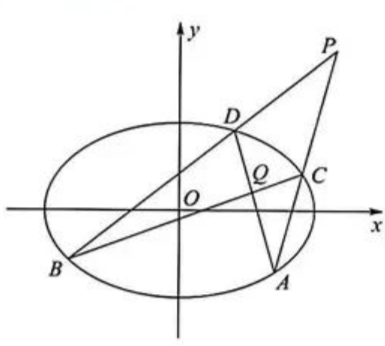
\includegraphics[width=0.6\textwidth]{flg/example.png}
%     \caption{导数的几何意义}
%     \label{fig:derivative}
% \end{figure}